%%%
%%%
\chapter{Warm-up: pigeonhole and numbers}
%%
%%%


%%%
\section{Pigeonhole principle}
%%%


Let me start with a question to you. 

\begin{exercise}
Last time I checked, there were 79 students enrolled in this course. Can anyone tell me if there is at least one pair of students whose birthday happen on the same week? Any guesses?
\SV[2021-08-17]{So my class has 46 right now... but let's keep them with this illusion}
\murmuno[08-24]{You can substitute your number during the lecture! Or even better, we can add up our numbers. Do you want me to change the numbers?}
\end{exercise}

In fact, I guarantee you, without knowing any of your birthdays, that yes. Moreover, I can guarantee that for some seven people in our class, their birthdays fall on the same month. And I am so sure of it because I can prove it using the ``pigeonhole principle''.

\begin{theorem}[Pigeonhole principle]
\label{thrm:pigeonhole}
If $k>0$ is a number of pigeonholes, and  $n$ pigeons try to occupy them, with $n>k$, then there will necessarily be a pigeonhole with at least two pigeons in it.
\end{theorem}

Here is a brief example with $k=9$ and $n=10$:\\
{\begin{center} 
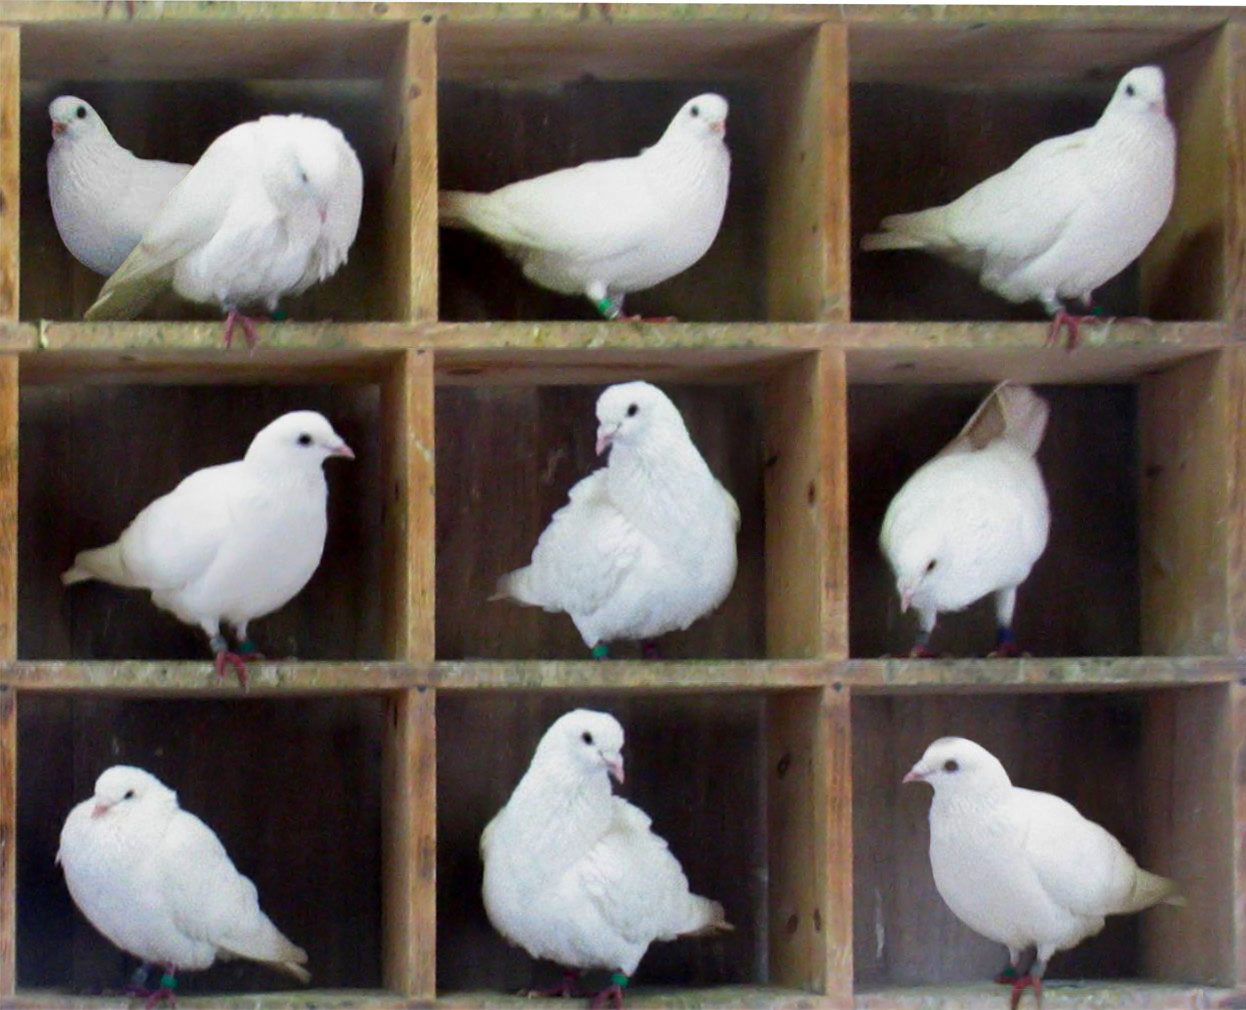
\includegraphics[width=0.4\textwidth]{pics/pigeonhole:TooManyPigeons.jpg}
\end{center}}

The statement sure seems obvious, but let us prove it as a warm-up, and then we'll use it to prove our first claim about birthdays.

\begin{proof}
We use a proof by contradiction.
Assume that none of the boxes has more than one item. Then we would only have at most $k$ items on our hands. But we assumed that the number of items is greater than $k$, so we arrived at a contradiction, and our assumption was false. So there must be a box with at least two items.
\end{proof}


\begin{example}
In a class of 79 students, there are at least two students whose birthdays fall on the same week.
\end{example}

\begin{proof}
Here the weeks in a year -- total of 52 -- play the role of pigeonholes, and students -- total of 79 -- play the role of pigeons.
\end{proof}

\begin{example}
There are two people in Pennsylvania with the same number of hairs on their body.
\end{example}

\begin{proof}
Possible numbers of hairs on a human body play the role of pigeonholes and people play the role of pigeons. By googling, we can find that people usually have 5 million hairs on their body and the population of Pennsylvania is 13 million. Therefore, by pigeonhole principle, there should exist at least two people with the exact same number of hairs.
\end{proof}

Now you may think that that was easy. Let us take it up a notch and see what happens when you have many more pigeons than pigeonholes.

\begin{theorem}[Generalized pigeonhole principle]
\label{thrm:gen_pigeonhole}
If $k>0$ is a number of pigeonholes, and $n$ pigeons try to occupy them, with $n>mk$ for some positive integer $m$, then there will necessarily be a pigeonhole with at least $m+1$ pigeons in it.

In other words, we can say that if $n$ pigeons occupy $k$ pigeonholes, then there is at least one pigeonhole containing at least $\lceil \frac{n}{k} \rceil$ items. The number $\lceil \frac{n}{k} \rceil$ is defined as the smallest integer that is larger than $\frac{n}{k}$.
\end{theorem}

\begin{exercise}
Prove Theorem \ref{thrm:gen_pigeonhole}.
\end{exercise}

\begin{example}
In a class of 79 students, there are at least seven students whose birthdays fall on the same month.
\end{example}

\begin{proof}
Here the months in a year -- total of $k=12$ -- play the role of pigeonholes, and students -- total of $n=79$ -- play the role of pigeons. Then we can calculate that $n = 6 \cdot k + 7$, so by the generalized pigeonhole principle (Theorem \ref{thrm:gen_pigeonhole}) there are at least $6+1 = 7$ students whose birthdays occur in the same month.
\end{proof}

\begin{example}
Pennsylvania needs to have at least two area codes for the phone numbers, while the US needs at least 42.
\end{example}

\begin{proof}
Phone numbers in the US have the format $+1 \, (AAA) \, N******$, where $AAA$ is the area code. The six stars are digits from 0 to 9, while $N$ can only be from 2 to 9. There are more subtle rules that you can find in Wikipedia on the page \href{https://en.wikipedia.org/wiki/North_American_Numbering_Plan#Modern_plan}{``North American numbering plan''}, but further restrictions do not affect the order of magnitude, so let us ignore them for now.
With this, the total possible number of variants to fill the stars is $8 \cdot 10^6 = 8\,000\,000$, so $k=8$ million. As we have found out before, there are $n = 13$ million people in Pennsylvania. So minimal number of area codes is $\lceil \frac{13}{8} \rceil = 2$.

The population of the US is $n=328.2$ million, so you will need at least $\lceil \frac{328.2}{8} \rceil = 42$ area codes.
\end{proof}

In fact, if you google, you will find out that major cities in any state have their own area codes, sometimes a couple, and the total number of area codes is now around 320. 

\begin{exercise}
Can you think of reasons to have so many area codes? (Logistical, social, etc.) Do you think there is a restriction on applying mathematical ideas in real life?
\end{exercise}



%%%
\section{Proving things with the pigeonhole principle}
%%%

Material for this section is take from
\url{https://www.math.uvic.ca/faculty/gmacgill/guide/pigeonhole.pdf}.

As we saw in the above examples, there are four steps involved:
\begin{enumerate}
    \item Decide what pigeons are. They will be the things among which we want to find several of that have the same property.
    \item Set up pigeonholes. In order for the pigeonhole principle to work, it is necessary to have fewer pigeonholes than pigeons. Sometimes you need an astute observation to do this.
    \item Give a rule for assigning the pigeons to the pigeonholes. The pigeonhole principle works for any rule -- you just need to choose the rule that works best for your situation.
    \item Apply the pigeonhole principle to your setup and get the desired conclusion.
\end{enumerate}

\begin{exercise}
Prove that if seven distinct numbers are selected from $\{1, 2,\dots, 11\}$ (braces are used to denote a \emph{set} of objects, e.g. numbers),
then some two of these numbers sum to $12$. Show that you can find six number so that no pair among those sums up to $12$. 
\end{exercise}

\begin{enumerate}
    \item Let the pigeons be the numbers selected.
    \item Let the pigeonholes be labeled by the following sets of numbers: $\{ 1,11 \}$, $\{ 2,10 \}$, $\{ 3,9 \}$, $\{ 4,8 \}$, $\{ 5,7 \}$, $\{ 6 \}$.
    \item The rule: when a number is selected, it is placed in the pigeonhole with the corresponding label.
    \item There are seven numbers and six pigeonholes, so two of the selected numbers will end up in the same pigeonhole. They cannot both end up in the pigeonhole labeled $\{6\}$ because we are choosing distinct numbers, so it's one of the first five. But then they sum up to $12$.
\end{enumerate}

\begin{exercise}
A party is attended by $n \geq 2$ people. Prove that there will always be
two people in attendance who have the same number of friends at the party. (Assume that
the relation ``is a friend of'' is symmetric, that is, if X is a friend of Y then Y is a friend of
X.)
\end{exercise}

Each person either is, or is not, a friend of each of the the other $n-1$ people in
attendance. Thus, the possible values for the number of friends a person can have in
attendance at the party are $0, 1,\cdots,n-1$. However, it can not be the case that there is
someone at the party with $0$ friends and someone else with $n-1$ friends simultaneously: if a person is
friends with everyone, then everyone at the party has
at least one friend there. Thus, the possible values for the number of friends a person can
have in attendance at the party are $0, 1,\cdots,n-2$ or $1, 2,\cdots,n-1$. In either case, there
are $n$ numbers (of friends among the people in attendance) that can take on at most $n-1$
different values. By the Pigeonhole Princple, two of the numbers are equal. Thus, some
two people in attendance who have the same number of friends at the party.

\section{Divisibility}

Let us now make things a little more abstract with numbers.
We will not concern ourselves with where numbers come from 
(although this is a worthy subject in itself)
but will learn how to do things with them.
In particular, we will spend some time thinking about
something that is very closely related to the pigeonhole principle: divisibility.

Let us first equip ourselves with a vocabulary.

\begin{itemize}
    \item \emph{Natural numbers} are numbers that are used for counting, starting
        from 0.
        We denote $\N$ to be the set of all natural numbers.
        Thus, using set notation\footnote{We will discuss sets later.},
        \begin{equation*}
            \N = \set{0,1,2,\dots}\,.
        \end{equation*}
    \item \emph{Integer numbers} are numbers that are used to measure the difference
        between two instances of counting.
        We denote $\Z$ to be the set of all integers.
        Thus, using set notation,
        \begin{equation*}
            \Z = \set{\dots, -2, -1, 0,1,2,\dots}\,.
        \end{equation*}
\end{itemize}

The shorthand of saying ``$a$ belongs to a set $S$ '' is by using the notation
\begin{equation*}
    a\in S \,.
\end{equation*}
For example, the shorthand of ``$a$ is an integer'' is ``$a\in \Z$''\,.

For what to come, we need the notion of the \emph{absolute value} of a number.

\begin{definition}
    The \emph{absolute value} of a number $a$ is a non-negative quantity 
    that represents the size of that number.
    In mathematical terms, 
    \begin{equation*}
        \abs{a} = 
        \begin{dcases}
            a \quad & \text{ if } a \geq 0 \,,  \\
            -a  & \text{ if } a < 0 \,. 
        \end{dcases}
    \end{equation*}
\end{definition}

Our strategy for uncovering the structure of the natural numbers is to break down complex objects and ideas into their fundamental components, think about this quote by Desmond Tutu, a South African Anglican cleric and theologian,
and a human rights activist\footnote{See also \url{https://www.psychologytoday.com/us/blog/mindfully-present-fully-alive/201804/the-only-way-eat-elephant}.}:
\begin{displayquote}
There is only one way to eat an elephant: a bite at a time.
\end{displayquote}
For example, when you prepare for an exam, you make a list of topics and learn one topic at a time; when I prepare lectures, I make a list of topics and write about one topic at a time; in both situations we achieve a complex result by taking many small bites. And when we study natural number, we break them down into their simplest building blocks -- \textit{prime numbers} -- and then study their properties and observe how they interact. One way of breaking the numbers down is to try to divide by a smaller number and observe if there is a remainder. This leads us to the following sequence of definitions.
    
\begin{definition}
    \label{def:divisibility}
    A number $a\in \Z$ is said to be \emph{divisible} by $b\in \Z$ if there exists 
   a number $q\in \Z$ such that 
   \begin{equation*}
       a = bq\,.
   \end{equation*}
   $b$ is called to be a \emph{divisor} (or a \emph{factor}) of $a$ and we can also say that $b$ \emph{divides} $a$ (notation: $b\st a$).

   The number $a$ is \emph{not divisble} by $b$ if $a$ can be written in the form 
   \begin{equation*}
       a = bq +r\,,
   \end{equation*}
   where $q,r \in \Z$ and $0<r<\abs{a}$. The number $r$ is then called the \emph{remainder}.
\end{definition}

    
    Just because I can define something, it doesn't mean that my definition is 
    something that makes sense.
    For example, I can define \emph{a cat} to be a mammal that lays eggs (what's wrong?).
    A good principle in life: question yourself often. Just because
    there are things you can imagine/define, it doesn't mean that those things exist
    or even make sense.

\begin{question}
    Does Definition~\ref{def:divisibility}  make sense? 
    Can there be a number that is both divisible and not divisible by another number?
\end{question}

There is a theorem that guarantees that the situation described in the previous question cannot happen.
In other words, Definition~\ref{def:divisibility} does make sense.

\begin{theorem}[Division theorem]
   Let $a,b \in \Z$ with $b\not= 0$.
   There exist a pair of integers $q,r \in \Z$ such that 
   \begin{equation*}
       a = qb + r \quad \text{ and } \quad 0 \leq r < \abs{b} \,
       ,
   \end{equation*}
   and moreover this pair is unique.
   $q$ is called the \emph{quotient} of $a$ when divided by $b$;
   and $r$ is called the \emph{remainder} of $a$ when divided by $b$.
\end{theorem}

\begin{example}
    Let $a = 101$ and $b = 3$. Then
    \begin{equation*}
        101 = 33\cdot 3 + 2 \,.
    \end{equation*}
    Here, $q =33$ and $r = 2$.
    As said in the division theorem, $2 < 3$.
\end{example}

\begin{example}
   A slightly interesting example is when $ a $ is positive and $b$ is negative.
   Say, $a = 23$ and $b = -4$. Then 
   \begin{equation*}
       23 = (-5) \cdot (-4) + 3 \,.
   \end{equation*}
   In this case $q = -6$ and $r = 3 < 4 $.
\end{example}

We will not prove this theorem for now as it uses the technique of mathematical induction (CS majors would say ``recursion'').

\begin{exercise}
    Read the proof of this theorem in Newstead's book~\cite{Newstead} (Theorem 6.1.1).
\end{exercise}



%%%
\section{Criteria of divisibility}
%%%

Numbers that are divisible by two are called \emph{even}, and they have a special name because in many cultures the distinction between odd and even numbers is quite prominent. For example, ancient Greek and Chinese seem to favor odd numbers like 3 and 5. Russian culture traditionally favors 3 and 7: there is a saying that ``God loves groups of three'', and seven commonly occurs in folk tales. Conversely, Eastern cultures have negative connotations with even numbers, and number 4 in Chinese is associated with death, because quite ominously, we can write it in two ways as an operation on two twos:
$$ 4 = 2\cdot 2= 2+2
.$$
Some buildings in China skip the fourth floor, just like the thirteenth floor is skipped in some places in the US.

On the other hand, Western cultures seem to ``prefer'' even numbers. According to a historian of mathematics (Dr. Nishiyama), ancient preference for odd numbers probably faded in the West with the arrival of modern mathematics as represented by Newton. When counting numbers, odd numbers were incomplete, in-between numbers, whereas even numbers were certainly more ``rational''. This is even reflected in an English proverb that says that two heads are better than one.

So how do we tell even numbers from odd?

\begin{proposition}
An integer number $n$ is divisible by $2$ if and only if its last digit is even (i.e. $0$, $2$, $4$, $6$, $8$).
\end{proposition}

\begin{lemma}
Observe that if a number $a$ is divisible by $b$, then $a + b$, $a + 2b$, etc. are also divisible by $b$. 
\end{lemma}

\begin{proposition}
An integer number $n$ is divisible by $5$ if and only if its last digit is $0$ or $5$.
\end{proposition}


\begin{proposition}
An integer number $n$ is divisible by $4$ if and only if its last two digits comprise a number divisible by $4$. An integer number $n$ is divisible by $8$ if and only if its last three digits comprise a number divisible by $8$. 
\end{proposition}

\begin{proposition}
An integer number $n$ is divisible by $3$ if and only if the sum of all its digits is divisible by $3$.
\end{proposition}

\begin{proof}
Prove the criterion of divisibility by 3 by writing the decimal expansion:
$$ a = a_k \cdot 10^k + \cdots + a_2 \cdot 100 + a_1 \cdot 10 + a_0 \cdot 1
.$$
Notice that $10^k = 9\dots9 + 1$, and the first summand is divisible by 3. So we can write
$$ a - 9\dots9 = a_k + \cdots + a_2 \cdot 100 + a_1 \cdot 10 + a_0 \cdot 1
.$$
Repeat this process and we can see that the right handside would eventually be 
\begin{equation*}
    a_k + \dots + a_1 + a_0 \,.
\end{equation*}
Note that
$a$ and each of the $9\dots 9$ is divisible by 3. Therefore, $a_k + \dots + a_0$ is divisible by 3.
\end{proof}

\begin{proposition}
An integer number $n$ is divisible by $9$ if and only if the sum of all its digits is divisible by $9$.
\end{proposition}

\begin{theorem}
    Let $n>70$ be a natural number that you want to test for being divisible by $7$.
    \\Step 1: Separate the last digit of the number, call it $d$.
    \\Step 2: Double the last digit and subtract from the remaining number, call the result $n_1$:
    $$ n_1 = \frac{(n - d)}{10} - 2 \cdot d
    .$$
    Then $n$ is divisible by $7$ if and only if $n_1$ is divisible by $7$. 
\end{theorem}
If after using this test once, you still get a number $n_1 > 70$, you can repeat the test and get some number $n_2$.

\begin{exercise}
    In 2019, a 12-year old Nigerian boy, Chika Ofili, suggested an alternative test for being divisible by $7$.
    Read the news article about Chika's test: \url{https://www.scilynk.in/divisibility-of-7/}.
    In this test, instead of subtracting $2d$, Chika suggests to add $5d$. What do you think about these two conclusions of the article?
    \begin{itemize}
    \item ``Multiplying by $5$ helps to reach a number within $0$--$70$ at a faster rate compared to multiplication by $2$.''
    \item ``Adding two numbers is psychologically simpler than subtraction.''
    \end{itemize}
    Test these conclusions on some numbers, e.g. 2021, 1234567: count the number of times you apply each test, and try to observe what is easier for you psychologically.
\end{exercise}

%%%
\section{Prime numbers}
%%%

When we factor numbers into smaller numbers, at some point we will have to stop, because there are some natural numbers that cannot be factored as the product of two smaller natural numbers. Trivially, zero and one are among them, but also there are 2, 3, 5, 7, 2017 and 2027.

I would like to argue that zero and one are so special that we don't even call them ``prime''. Most early Greeks did not even consider 1 to be a number, so they could not consider its primality. In modern mathematics, we actually have a formal definition that excludes 0 and 1 as prime numbers.

\begin{definition}
    A natural number $p$ is called prime if it has exactly two positive distinct divisors.
\end{definition}

With this definition, we can observe that 0 and 1 are not prime, because 0 is divisible by any number, while 1 is divisible by only one number -- 1 itself.

\begin{theorem}[Fundamental theorem of arithmetic]
    Every natural number $n>1$ is either a prime or it can be expressed as a product of prime numbers in a unique way.
\end{theorem}

\begin{proof}[Sketch of proof]
We will not prove this theorem because it requires a technique called induction, 
which we have not yet covered.

However, you should be able to see that the existence of such expression is simply 
a matter of definition. If a number cannot be factored into products of smaller number,
by definition, it is a prime number. Keep factoring the smaller number in the products until you get all primes.

The uniqueness part is the tricky part!
\end{proof}

\begin{remark}
   An important idea here is that in mathematics, a proof of unique existence of something
   is often done by two separate steps that are not in any order.
   Existence step is to establish that there is at least one object that satisfies the definition. 
   Uniqueness step is to establish that if two objects with the same definition exist,
   they must be the same.
\end{remark}


\begin{example}
We can first try and factor $2021$. Let's see which prime numbers, starting from the smallest, can divide it: not 2, 3, 5, 7... Eventually, we see that
$$ 2021 = 43 \cdot 47
.$$

Now let us do the same with $2020$. It is divisible by $2$, because its last digit is divisible by $2$:
$$ 2020 = 2 \cdot 1010 = 2^2 \cdot 505 = 2^2 \cdot 5 \cdot 101
.$$
\end{example}

While doing prime decomposition and testing which numbers are prime, you can observe that if $n$ is a natural number that is not divisible by any number up to $\sqrt{n}$, then $n$ is prime.

Sieve method for finding prime numbers.

\begin{theorem}
    There are infinitely many prime numbers.
\end{theorem}
\begin{proof}
    We prove this statement by proof by contradiction. 
    
    Suppose that there are only finitely many primes, listing them as\footnote{
    Note that it is necessary for a finite list of number to have a largest number and a
    smallest number.
    In this case, the largest number in our prime list is $p_n$.
    }
    \begin{equation*}
        p_1 < p_2 < \dots < p_n \,.
    \end{equation*}
    

    Then we claim that the number 
    \begin{equation*}
        a = p_1p_2 \dots p_n + 1 
    \end{equation*}
    is a prime number, which is larger than the largest prime number $p_n$, a contradiction.
    To see that $a$ is a prime number, we suppose that it is not a prime number, then 
    it must be uniquely factorizable by  the primes from $\set{p_1,\dots, p_n}$.
    In particular
    \begin{equation*}
        a = p_{l_1}^{m_1} \cdot \dots \cdot p_{l_k}^{m_k} \,.
    \end{equation*}
    But then we have 
    \begin{equation*}
        1 = p_{l_1}\cdot \dots \cdot p_{l_k} 
        ( p_{l_1}^{m_1-1} \cdot \dots \cdot p_{l_k-1}^{m_k-1} - q ) \,,
    \end{equation*}
    where $q$ is some natural number.
    This is a contradiction because that means both
   \begin{equation*}
       p_{l_1}\cdot \dots \cdot p_{l_k}
   \end{equation*} 
   and 
   \begin{equation*}
       ( p_{l_1}^{m_1-1} \cdot \dots \cdot p_{l_k-1}^{m_k-1} - q )
   \end{equation*}
   must be $1$ or $(-1)$.
   This is impossible as at least
   $ p_{l_1}\cdot \dots \cdot p_{l_k} > 1$ by definition of primes.
\end{proof}

\begin{remark}
   The proof above is by Euclid in 300 B.C.. A remarkable feat! 
\end{remark}

\begin{exercise}
    Infinity is lurking behind us already. You should start asking yourself what
    infinity really is and try to come up with a definition on your own.
\end{exercise}
%%%
\section{Greatest common divisor}
%%%


One of the most fundamental concepts about numbers is the greatest common divisor.

\begin{definition}
    Let $a, b \in \Z$. An integer $d$ is a \emph{greatest common divisor} of $a$ and $b$
    if:
    \begin{enumerate}
        \item $d \st a$ and $d \st b$,
        \item  if $q$ is another integer such that $q\st a$ and $q \st b$ then
            $q \st d$.
    \end{enumerate}
    We denote the (unique) non-negative greatest common divisor of $a$ and $b$ as $\gcd(a,b)$.
\end{definition}

\begin{exercise}
    Why is it that in our definition, we have ``a'' greatest commond divisor, 
    but not ``the'' greatest common divisor?
\end{exercise}

\begin{theorem}
   Let $a,b,q,r \in \Z$ and suppose that $a = qb + r$. Then
   \begin{equation*}
       \gcd(a,b) = \gcd(b,r) \,.
   \end{equation*}
\end{theorem}
\begin{proof}
    First, note that any number $c$ that divides both $a$ and $b$ also divides $r$.
    To see this, we can write $a = m_1 c$ and $b= m_2 c$.
    Therefore, 
    \begin{equation*}
        m_1 c = q m_2 c + r \,,
    \end{equation*}
    which is equivalent to
    \begin{equation*}
        r = c (m_1 - q m_2)\,.
    \end{equation*}
    By definition, $c$ is a divisor of $r$.


    Second, if $d$ divides both $b$ and $r$ then $d$ divides $a$. 
    To see this, we write $b = m_3 d$ and $r = m_4 d$.
    Therefore,
    \begin{equation*}
        a = q m_3 d + m_4 d = (q m_3 + m_4m) d \,.
    \end{equation*}
    
    By those two observations, and definition of greatest common divisor,
    \begin{equation*}
        \gcd(a,b) \leq \gcd(b,r) \quad \text{ and } 
        \quad \gcd(a,b) \geq \gcd(b,r) \,.
    \end{equation*}
    This means that 
   \begin{equation*}
       \gcd(a,b) = \gcd(b,r) \,,
   \end{equation*}
   as desired.
\end{proof}



One question arise, how can we find the greatest common divisor of any two numbers?
For example, how on earth are we supposed to know $\gcd(199888,4987774)$?
Luckily, ancient people were pretty smart and there is a method that was invented
at least 2300 years ago as it first appeared in Euclid's Elements (300 BC).
We, as modern people, still benefit from this method as it has a lot of practical applications~\footnote{For a curious mind, you can read more about it here: \url{https://en.wikipedia.org/wiki/Euclidean_algorithm}}.

\begin{theorem}[Euclid's algorithm]
    Let $a,b \in \Z$. The $\gcd(a,b)$ is computed as follows.
    \begin{itemize}
        \item Set $r_1$ to be the remainder of $a$ divided by $b$ .
        \item Set $r_2$ to be the remainder of $b$ divided by $r_2$.
        \item Given $r_{n-2}$ and $r_{n-1}$, define $r_n$ to be 
            the remainder of $r_{n-2}$ divided by $r_{n-1}$.
        \item Stop when $r_{n+1} = 0$; then $r_{n} = gcd(a,b)$.
    \end{itemize}
\end{theorem}
Writing everything explicitly, we have
   \begin{gather*}
       a = bq_1 + r_1 \qquad ( 0< r_1 < b)\\ 
       b = r_1q_2 + r_2 \qquad ( 0< r_2 < r_1)\\ 
       r_1 = r_2 q_3 + r_3 \qquad ( 0< r_3 < r_2) \\
       \dots \\
       r_{n-2} = r_{n-1} q_{n} + r_n \qquad ( 0< r_n < r_{n-1}) \\
       r_{n-1} = r_n q_{n+1} + 0  \,.
   \end{gather*}
Then $\gcd(a,b) = r_n$.

\begin{exercise}
   Why must there is a $0$ remainder at the end of Euclid's algorithm?
   This is an important question because it answer the following question,
   ``why should the algorithm stop?''
   Is there a scenario when you have to do this forever?
\end{exercise}

\begin{example}
   Use Euclid's algorithm to find
   \begin{equation*}
       \gcd(242, 66)\,.
   \end{equation*}
    Let's compute!
    \begin{gather*}
       242 = 66\cdot 3 + 44\\
       66 = 44\cdot 1 + 22\\
       44 = 22\cdot 1 + 0\,.
    \end{gather*}
    So $\gcd(242,66) = 22$.
\end{example}


Let's have some fun with greatest common divisors using Euclid's algorithm.
\begin{corollary}
    Let $l = \gcd(a,b)$. Then there exist two integers $m,n$ such that
    \begin{equation*}
        l = am + bn\,.
    \end{equation*}
\end{corollary}
\begin{proof}
   We apply Euclid's algorithm to prove this statement. 
   Writing everything explicitly, we have
   \begin{gather*}
       a = bq_1 + r_1 \qquad ( 0< r_1 < b)\\ 
       b = r_1q_2 + r_2 \qquad ( 0< r_2 < r_1)\\ 
       r_1 = r_2 q_3 + r_3 \qquad ( 0< r_3 < r_2) \\
       \dots \\
       r_{n-2} = r_{n-1} q_{n} + r_n \qquad ( 0< r_n < r_{n-1}) \\
       r_{n-1} = r_n q_{n+1} + 0  \,.
   \end{gather*}
   We know that, $l = r_n$ because that is the content of Euclid's algorithm.

   Now, to show what we want to show, we reverse engineer what's happening.
    Rewriting 
    \begin{equation*}
        r_1 = a - bq_1\,.
    \end{equation*}
    Then,
    \begin{equation*}
        r_2 = b - r_1 q_2 = b - (a + b q_1)q_2 = (1 - q_1q_2) b - q_2 a \,.
    \end{equation*}
    Keep doing this until $r_n$ and we will arrive at our conclusion.
\end{proof}

